\chapter{Evaluating the Effect of Homicide Prevention Strategies in São Paulo, Brazil: A Synthetic Control Approach}
\label{chap:synth}

\section{Introduction}

Brazil has long been ravaged by an undeclared civil war. According to the Citizen Council on Public Security and Criminal Justice, a Mexican think-tank, 19 of the 50 most violent cities in the world are located in Brazil \citep{mexico2014}.\footnote{The study disregards war zones and cities with unavailable data.} The 2014 Violence Map survey shows that 56,337 people were murdered in Brazil in 2012 alone, the highest incidence rates of intentional homicides on the planet \citep{mapa2014, unodc2013}. Paradoxically, the sharp rise in lethal violence has occurred during Brazil's longest period of political openness \citep{ahnen2003, pinheiro2000, pinheiro2001}. Murder rates have almost doubled over three decades of democracy, jumping from 15 homicides per 100,000 people in 1985 to roughly 29 per 100,000 in 2012 \citep{mapa2014}.\footnote{\citet{cerqueira2013} argues that the actual rates may be different from the official statistics. He states that many homicides from 1996 to 2010 were (intentionally or not) misclassified as `death by undetermined causes.' After performing data correction procedures, the author estimates that the number of homicides in Brazil during that period should be 18.3\% higher than the reported figures. Recent criticism about the quality of São Paulo homicide data can also be found at \url{http://goo.gl/x0pHac} (in Portuguese). Access: January, 2016. In this article, I avoid these issues by using obituary data instead of police records.}

São Paulo has traditionally occupied a key position in Brazil's violence statistics. It is the country's richest and most-densely populated state, and in the 1990s its homicide rate was roughly 50\% higher than the national average \citep[120]{barata2000}. Some areas of the namesake capital city had even worse numbers. Between 1996 and 1999, the ramshackle districts of Jardim São Luiz and Jardim Ângela had respectively 103 and 116 violent deaths per 100,000 residents \citep[8]{cardia2003}, figures that placed them amongst the deadliest neighbourhoods on the globe \citep{who2015}.

Nevertheless, the state of São Paulo has experienced a drastic reduction in homicides during the last years \citep{camargo2007}. The decline is so remarkable that some authors have called it `the great homicide drop' \citep{goertzel2009}. The city of São Paulo, which is currently home to about 11 million inhabitants, provides a telling example. Over a span of only seven years (2000--2007), the number of annual violent deaths in the capital fell from 5,979 to 1,311, a 78\% decrease.\footnote{The homicide statistics cited in this paragraph come from the Centre for the Study of Violence, a research group of the University of São Paulo. Their data set can be found at the following electronic address: \url{http://nevusp.org/downloads/bancodedados/homicidios/distritossp/num-homicidios-distritos-2000-2007.htm}. Access: March, 2016.} Significantly, São Paulo city became the safest state capital in Brazil \citep{mapa2011}.

São Paulo's success should be attributed to local factors. From 1999 onwards, the state government created or expanded a number of policies that have arguably contributed to the decrease in criminality. In a move coherent with the basic tenets of the economics of crime \citep[e.g.][]{becker1968crime, cornish2014reasoning}, the administration increased the certainty and the intensity of punishment to discourage potential offenders. Amongst other measures, the government implemented strict gun control policies \citep{goertzel2009}, raised incarceration rates \citep{salla2007}, and imposed harsher sentences on those convicted of a crime \citep{carvalho2005}. 

But whereas several authors acknowledge the effectiveness of these policies, few quantitative studies have gone beyond statistical correlations to justify their arguments. In the case of São Paulo, a major difficulty is separating the state's particular time trend to that of Brazil. Ideally, one should compare São Paulo to a control case that shares the same characteristics of the existing state, except that it has not been subjected to the specific set of policies implemented by the São Paulo state government. This thought exercise, which emulates the logic of a controlled experiment \citep{angrist2008mostly, imbens2015causal, holland1986, morgan2014counterfactuals}, would allow practitioners to untangle the effects of homicide reduction programmes from other potential confounders. 

In this paper, I employ the synthetic control method (henceforth SCM) to approximate this experimental ideal and measure the total causal effect of post-1999 public policies on São Paulo homicide rates. The method consists of creating an artificial counterfactual to estimate the impact of a given intervention on a unit of interest. SCM has gained widespread acceptance in many fields, having been successfully applied in political science \citep{abadie2014, montalvo2011}, economics \citep{billmeier2013, coffman2012, jinjarak2013}, education studies \citep{hinrichs2012}, and public health science \citep{heim2014}. However, SCM has rarely, if ever, been used to evaluate homicide prevention strategies in São Paulo, despite being a useful tool for this particular type of question. SCM was specifically designed for situations where there is only one treated unit of interest, no readily-available counterfactual, and no certainty as to whether the treated and the control units follow parallel trends after the intervention \citep{abadie2003, abadie2010, abadie2014}. Moreover, SCM also has some of the desirable properties of popular causal inference tools such as differences-in-differences \citep{angrist2008mostly, bertrand2004much} and matching estimators \citep{dehejia2002propensity, ho2007matching, rubin1973matching, stuart2010matching}. 

I find that from 1999 to 2009, about 20,000 lives were saved in São Paulo. When compared to a synthetic counterfactual, São Paulo's actual homicide rates were less than 50\% of what would be expected in the absence of policy implementation (15 versus 32 homicides per 100,000 people). Additional tests confirm the robustness of the results and indicate a 96.3\% chance of a causal effect in the intervention period. 

The article is structured as follows. Section~\ref{sec:theoretical_background} discusses how deterrence provides a useful framework to understand the reduction in homicide rates in the state. I also examine an alternative hypothesis for the drop in crime in São Paulo -- the rise of the \emph{Primeiro Comando da Capital} -- and argue that the prison gang should be regarded as a moderator, but probably not as an independent cause of homicide reduction. Section \ref{sec:methods} presents a justification for, and a technical explanation of, the synthetic control method. Section \ref{sec:data} describes the data used in this paper. Section \ref{sec:analysis} discusses the results of the models and presents several robustness tests. Section \ref{sec:conclusion} offers some concluding remarks.

\section{Theoretical Background}
\label{sec:theoretical_background}

\subsection{Deterrence, Information and the Drop in Homicides}
\label{sub:deterrence_and_the_drop_in_homicides}

A myriad of explanations have been proposed for the fall in homicide rates in São Paulo. Some authors have stressed the importance of long-term factors on local levels of violence. \citet{mello2010} claim that the shrinking of the proportion of males in the 15--25 age bracket has led to fewer violent deaths at both state and city levels. \citet{hughes2004} argues that São Paulo's spatial segregation patterns have had a lasting impact on murder rates. \citet{barata2000}, in turn, posits that macroeconomic conditions, mainly inequality indicators, are positively correlated with violent crime in São Paulo.

Structural variables have likely been important in reducing violence, but the role of public policies should not be underestimated. The Brazilian Social Democracy Party (\emph{Partido da Social Democracia Brasileira}, PSDB), which has ruled São Paulo since 1995, has repeatedly asserted its commitment to reducing urban crime throughout the state \citep{bueno2014}. In 1998, former governor Mário Covas -- then running for re-election -- set the ambitious goal of ``slashing criminality rates in half'' during his second term in office \citep{santos2008}. This commitment was then followed by his vice-governor and successor, Geraldo Alckmin, who has expanded those measures and taken a notoriously tough stance on crime \citep{de2012governo}. 

Methods of crime prevention have received considerable attention from the authorities. Firstly, the São Paulo government significantly increased incarceration rates in the past decade \citep{salla2007}. The state currently holds around 200,000 convicts in prison (35\% of Brazil's inmate population) and adds another 15,000 inmates to the official statistics every year \citep{brasildefato2013}. Furthermore, prisoners have also become subject to harsher legal punishments. The São Paulo administration has also been making large use of the \emph{Regime Disciplinar Diferenciado} (Special Disciplinary Regime), which provides for up to 360 days of solitary confinement for disobeying the law \citep{carvalho2005}.

Secondly, the state government has successfully enforced a ban on gun possession in São Paulo. Studies show that this policy has been effective in reducing homicides resulting from both drug-related crimes and domestic disputes \citep{goertzel2009, kahn2005papel}. Furthermore, the impact of the Brazil's 2003 National Disarmament Act was particularly pronounced in São Paulo. \citet{cerqueira2013evaluating} argue that between 2005 and 2007 the enforcement of the anti-firearm legislation was responsible for saving between 2,000 to 2,750 lives in cities with more than half a million inhabitants in the state of São Paulo. 

This set of policies is largely in line with the rational choice theory of crime \citep[e.g.][]{becker1968crime, ehrlich1973participation,levitt1996effect, levitt1997using, paternoster2010much}. The rational choice school posits that criminals are motivated by utilitarian cost-benefit analysis. Individuals calculate what the possible trade-offs are between the benefit of the committing a crime and the risk of being punished for it. Criminal offenders, therefore, are in no way different from non-criminals: the only difference between them is their \emph{choices} \citep{nagin2007moving}. To reduce criminality, policy-makers have to ensure that the costs of committing a crime outweigh the eventual utility an individual derives from it.

Deterrence measures have been complemented by investments in police intelligence. In 1999, the state administration created a new system for crime prevention, Infocrim \citep[3]{risso2014intentional} The system gathers geo-coded information on homicides and maps the most important `hot spots' of criminal activity in the state. The government has also developed a new photo database, Fotocrim, to speed up the process of facial recognition of criminals \citep[3]{mello2010}. 

More information improves the effectiveness of police strategies via two mechanisms. On the one hand, police forces can be quickly moved to where they are most needed. This reinforces the role of deterrence as it increases the likelihood of punishment for criminals. On the other hand, the system also makes clear what regions are making progress in reducing crime. This allows police chiefs to monitor local personnel and take measures to improve performance if required.\footnote{See: \url{http://goo.gl/kqLhYb} (in Portuguese). Access: August 2016.} 

Recent evidence shows that the intelligence system has effectively lowered the crime statistics in São Paulo. Using a spatial differences-in-differences estimator, \citet{cabral2016infocrim} argues that Infocrim has had a large negative impact on homicide rates in the municipalities where it was implemented. The author also notes that the effect remains important even after accounting for possible displacement effects. As expected, some criminals did take their activities elsewhere after the creation of Infocrim, but this movement has not offset the benefits of the system.

How well have these policies performed over time? The results suggest a favourable outlook. Compared to other Brazilian states, São Paulo is an outlier when it comes to homicide rates. Despite the fact that crimes against property have declined little over the last decades,\footnote{Recent data on property crimes in São Paulo can be seen at \url{http://www.ssp.sp.gov.br/novaestatistica/Pesquisa.aspx} (in Portuguese). Access: July 2016.} the number of violent deaths per 100,000 inhabitants shows a steep downward trend. Figure \ref{fig:figure1} presents the evolution of homicide rates in São Paulo in comparison with the Brazilian average.

\begin{figure}[H]
    \centering
    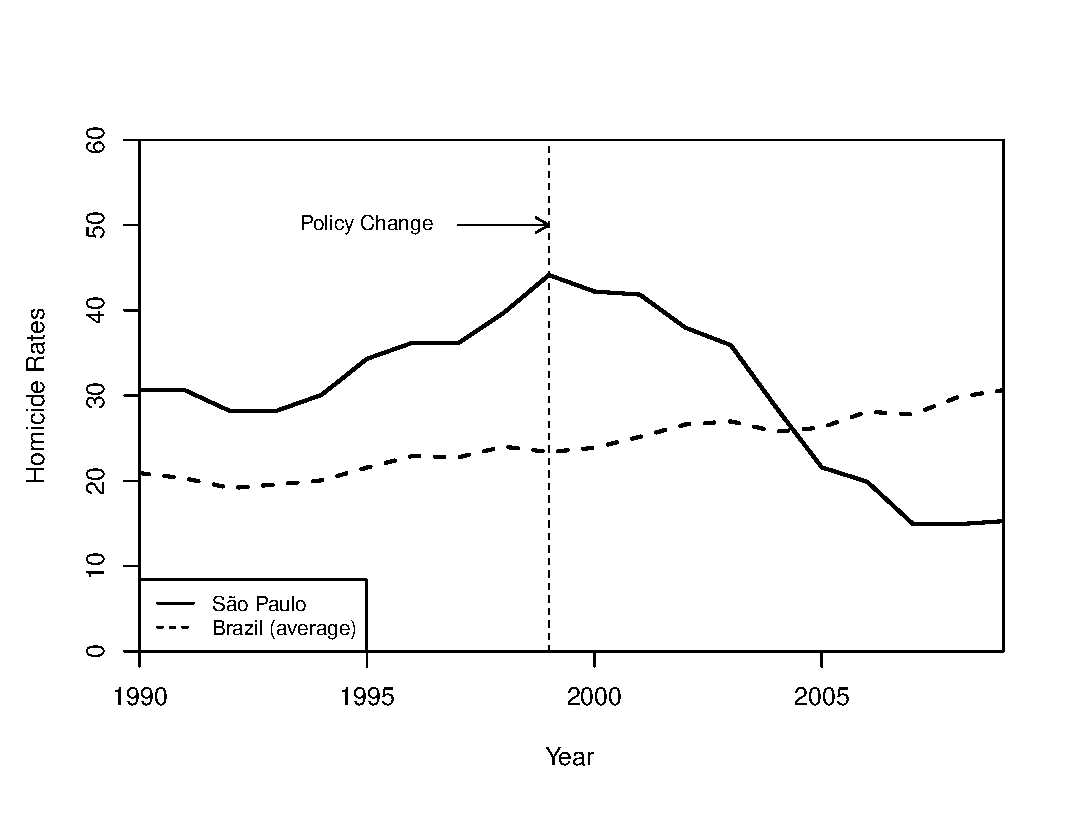
\includegraphics[height=7.5cm]{images/br.eps}
    \caption{Homicide Rates per 100,000 Population -- São Paulo and Brazil (Excluding São Paulo)}
    \label{fig:figure1}
\end{figure}

The trends are even more striking if we consider that deterrence policies are still controversial in the literature. \citet{barbarino2014incapacitation}, \citet{buonanno2013incarceration}, \citet{levitt1996effect,levitt2004understanding} and \citet{owens2009more} claim that incapacitation measures effectively reduce crime, but \citet{eck2006have} and \citet{beattie2007police} suggest that increases in police forces and incarceration rates in the United States and in Canada did not lead to expected outcomes. 

There is good evidence that incapacitation measures have worked well in São Paulo during the last decade. Gun-related homicides have declined about 74\% from 2001 to 2008 \citep{peres2011queda} at the same time when São Paulo has experienced an increase of 770\% in the arrests of repeated murderers \citep[36]{manso2012homicidos}. Although there are studies that indicate possible `hardening effects' of imprisonment, that is, longer sentences may positively affect an individual's tendency to commit further crimes \citep[e.g.][]{chen2007harsher,glaeser1996crime,western2001labor}, the São Paulo case appears to suggest otherwise. Moreover, violent deaths have decreased in all population strata, but especially amongst males (-74.5\%), 15 to 24 year-old men (-78,0\%) and those who live in extreme poverty (-79,3\%), groups that are generally associated with criminality \citep{peres2011queda}.

Nevertheless, it is difficult to know which of the policies have contributed more to this large homicide reduction. Not only we do not have disaggregated data to test preliminary hypotheses, but there may be large interaction effects amongst different public security measures. Therefore, at the moment it is not possible to disentangle micro-level causes from macro effects. But the aggregated impact of the anti-crime policies can be correctly identified if there is no other variable in the causal path leading from the policies mentioned above to our dependent variable (state homicide rates). I argue below that this type of estimation is feasible for the São Paulo case. To back this claim, I suggest that a competing explanation for the homicide drop in São Paulo -- the rise of the PCC -- interferes only with the direct effect of the policies on crime, but not with their \emph{total} effect. In this sense, the synthetic control method provides a plausible identification strategy for my question of interest.

\subsection{Alternative Explanation: The Emergence of the PCC}
\label{sub:alternative_explanation_the_emergence_of_the_pcc}

A recent hypothesis attributes the decrease in violent deaths in São Paulo to the \emph{Primeiro Comando da Capital} (First Command of the Capital, henceforth PCC) \citep{biondi2010, dias2009, dias2011pulverizaccao, de2010crime, de2012governo, willis2015killing}. The PCC is a prison gang that emerged in the early 1990s as a response to the demands of a growing prison population. The PCC provides personal security and financial assistance to their members and affiliates. The gang's internal statute clearly declares that ``[\dots] those who are in liberty [must contribute] to the brothers inside prisons [PCC members] through lawyers, money, help to family members and prison outbreak operations'' \citep{folha2001estatutopcc}.

A group of scholars argue that the PCC significantly contributed to the reduction in violence mainly through the São Paulo prison system. At least since the mid-2000s, these authors argue that the PCC has been able to emerge as an undisputed mediator and solve conflicts between inmates. \citet[83]{dias2009ocupando} writes that ``[\dots] when unable to constitute a universal source of regulation, the official law leaves gaps which are filled by informal instances -- such as the Primeiro Comando da Capital (PCC), in the prisons of São Paulo.'' The gang has implemented informal courts that resemble state institutions, and those meetings have progressively replaced other forms of popular justice such as lynchings or the hiring of target killers \citep[3]{feltran2012metodos}. Moreover, the \emph{Comando} has developed a series of assertive ways to terrorise inmates. Since the PCC's threats are credible, the group is able to impose discipline within the São Paulo prison system \citep{biondi2010,dias2009}.

Paradoxically, the PCC might have also helped to reduce crime in São Paulo by collaborating with street-level police. The Brazilian state does not hold a perfect monopoly of force in many areas of the country \citep{arias2009drugs,de2012governo,hughes2004,pinheiro2000}, thus access to local knowledge may prove vital for the success of a given operation. In this regard, the PCC and the state may collude if the situation is beneficial to both, and as such there is an informal--but potentially unstable--``killing consensus'' in the state \citep{willis2014antagonistic, willis2015killing}.

There has been a vigorous debate over whether the PCC has had a significant impact on violence rates. A few authors see the PCC as the sufficient condition behind the homicide rates decline across São Paulo state \citep{biondi2010, dias2009, dias2011pulverizaccao}, whilst others take a more nuanced view of the role of the prison gang \citep[e.g.][]{willis2015killing}. But both groups of scholars affirm that, based on their first-hand experience, the PCC is the key explanatory variable behind the drop in murders in São Paulo.

Recent econometric works, however, do not seem to confirm that argument. Marcelo Nery has found no convincing results in favour of the `PCC hypothesis' using geo-referenced data for São Paulo \citep{bbc2016pcc}. \citet{biderman2015pax} use anonymous calls to a crime hotline as a proxy for PCC presence in São Paulo city favelas. The authors suggest there is some support for the idea that the criminal syndicate reduces lethal violence in areas under its control, but PCC presence corresponds to only a minor drop in violent crime. Although the PCC impact is not negligible, the gang is not a sufficient condition for the homicide decline.

Another counter-argument to the PCC thesis is that homicides also decreased in areas and groups over which the PCC does not exert control. Firstly, descriptive statistics show that the decline in violent deaths started \emph{before} the PCC's expansion period.\footnote{As shown in figure \ref{fig:figure1}, São Paulo's homicide rates started to drop in 1999. The PCC consolidated their power in the prison system only in the mid-2000s \citep{dias2011pulverizaccao}.} Secondly, the drop in crime was evenly distributed throughout the state: urban and rural areas, small and large cities alike experienced fewer murders.\footnote{See: \url{http://www.fenapef.org.br/27764/} (in Portuguese). Access: July 2016.} Finally, as noted above, \citet{peres2011queda} point out that violent death rates decreased in \emph{all} age groups and social classes in the city São Paulo. Hence, cohorts that do not correspond to typical PCC members (such as the elderly or middle-age females) are also less affected by violence. 

It seems that the influence of the PCC on physical violence has been overstated. It is unlikely that the PCC -- which is underfunded for its size\footnote{A Parliamentary Commission of Inquiry has stated that the PCC earns about 16 million Brazilian Reals per month, which amounts to approximately 60 million US dollars per year. See: \url{http://goo.gl/FwhPa3} (in Portuguese). Access: July 2016. Given the size of the organisation and its undisputed position as the leading crime syndicate in São Paulo, the figures are rather small. As a comparison, Mexico's Sinaloa Cartel profits about 3 billion dollars per year, a sum comparable to the annual earnings of Netflix or Facebook. See: \url{http://nyti.ms/1B09qyV}. Access: July 2016.} -- could have achieved such deep penetration into society and lowered the violence levels across all population groups in the whole state. 

Yet, the group's importance cannot be fully dismissed either. Data on PCC-controlled areas are likely to contain measurement errors that may bias the coefficients, thus caution is required before making strong causal claims on this discussion. Despite mounting observational evidence that the PCC may not provide a complete explanation to São Paulo's lower crime rates, the argument could only be comprehensively tested in a counterfactual case in which the PCC is present and the state policies are not.\footnote{I would like to thank an anonymous reviewer for highlighting this point.} Currently-available data do not allow us to evaluate such scenario.

\subsection{Causal Paths, Moderators, and Total Effects}
\label{sub:causal_paths_moderators_and_total_effects}

A methodological issue remains. If we are to estimate the causal effect of the public measures on the crime rates, how should we proceed? I have noted above that the specific impact of micro-level policies cannot be evaluated due to lack of data. Nonetheless, it is theoretically possible to estimate the \emph{total} effect of policies on crime. 

The difference between direct and total effects can be understood as follows. The direct effect captures the sensitivity of a dependent variable $Y$ to changes in $X$ when this relationship is not mediated by any other variables in the model. Holding all factors constant, the direct effect is a causal chain of length one \citep[160]{sobel1987direct} and could be described simply as $X \rightarrow Y$. In turn, the total effect can be defined as $P(Y_{x} = y)$, that is, ``the probability that response variable $Y$ would take on the value $y$ when $X$ is set to $x$ by external intervention'' \citep[1572]{pearl2001direct}. The total effect is the sum of direct and indirect (or mediated) effects. 

In our case, gun control, incarceration, and police intelligence have likely had a direct effect on homicides. Combined, these variables comprise a direct aggregate policy effect. The omission of a variable measuring the impact of the PCC could bias such an effect, but not interfere with the \emph{total policy effect}. This point is worthy of further consideration. The total policy effect would be unbiased under the assumption that the PCC is in fact a \emph{moderator} between the public policies and the homicide rates, even if the gang's impact over the violence levels is not particularly large. 

Although this argument has rarely been posited in such terms, this position is largely supported by the qualitative literature on the PCC. Fieldwork research generally traces the group's origins and growth to the rising incarceration rates in São Paulo and the need for protection amongst prisoners \citep{dias2011pulverizaccao, manso2014}. Like other prison groups, the PCC would only mobilise resources to provide welfare and act as an arbitrator under the condition that the certainty of punishment by the state is high \citep{skarbek2011, freire2014}. Had the state not increased the costs associated with crime, the prison gang would not have expanded their reach, or even been created in the first place. Hence, the impact of the PCC on street-level violent deaths -- if it exists -- can be safely assumed to be a moderator effect. 

Whereas it would be interesting for researchers to separate these types of effects and isolate the PCC from the other causal outcomes, such estimation is not possible at the state level. However, as these measures were implemented throughout São Paulo state at roughly the same time, their combined effect is computable even though their individual direct effects are not. To do so, it is only necessary to contrast the treated unit (São Paulo) with a counterfactual without the time-assigned treatment (1999 onwards) and evaluate the aggregated effect of the public policies.

This analysis can be estimated in a consistent manner with the synthetic control method. In the following sections I describe how the method creates a valid counterfactual case under a certain set of assumptions. The assumptions are: 1) the PCC is an outcome, not a cause, of the crime-targeting policies; 2) the model does not include unnecessary control variables; 3) interpolation bias is not very severe because the cases in the `donor pool' are relatively similar to the treated unit. 

\section{Methods}
\label{sec:methods}

The synthetic control approach provides an adequate solution for two enduring problems in the social sciences: the arbitrary selection of comparative cases and the poor estimation of causal effects when few pre-treatment observations are available \citep{abadie2003, abadie2010}. With respect to the first issue, scholars often resort to ambiguous criteria in their choice of control units. This practice ends up casting doubts over the validity of their selected counterfactual \citep{abadie2011}. The synthetic method provides a reliable comparative case by adopting a purely data-driven process in order to select a counterfactual. Also, the researcher can still specify what control cases enter the `donor pool.' In this sense, qualitative expert knowledge can be incorporated in the estimation via the selection of cases. 

Regarding the second issue, the accurate estimation of coefficients from a small number of cases, SCM employs a consistent statistical solution to problems of incorrect data extrapolation and model dependence. SCM can be understood as a combination of matching with differences-in-differences. SCM uses matching as a flexible pre-processing tool to reduce imbalance between treated and control units \citep{ho2007matching, rubin1973matching, rubin2006matched}. But unlike matching, SCM deals with only one treated unit over time. Therefore, the method can also be interpreted as a semi-parametric extension to differences-in-differences estimators in which both treated and control units are not required to follow parallel trends in the whole period. \citep{abadie2005semiparametric}. By combining semi-parametric matching with differences-in-differences, SCM provides a rigorous yet versatile method to evaluate time-dependent treatment effects. 

The method works as follows.\footnote{Please refer to Appendix~\ref{sec:synth-appendix} for a formal presentation of the synthetic control method.} SCM starts with the assumption that one case in the sample has received a treatment. The treatment is defined as a time-delimited event that affects the unit of interest, such as the implementation of a new policy or the outbreak of a conflict. SCM also requires a series of control cases to estimate the models, that is, units that did not receive the treatment during the same period. These cases are often related to the treatment case in some meaningful way, and natural choices for the donor pool are provinces within the same country, or states that share important characteristics. These traits can also be more specifically defined and included as quantitative variables in the estimation models. 

SCM then selects a few cases from the donor pool to create a new, artificial control for the treated unit of interest. The main goal of SCM is to construct a counterfactual that resembles the treatment unit more closely than any individual control in the donor pool. Cases are combined in way similar to a weighted average, in which controls that are more similar to the treated unit receive more weights. The weights make explicit the contribution of each separate case to the synthetic control, what also increases the transparency and reliability of the method \citep{abadie2014}. The closer the synthetic control matches the original treated unit before the assignment of the period, the better the quality of the counterfactual. 

The method uses an algorithm to minimise the difference between the control cases and the treated unit before the intervention. The authors adopt the mean squared prediction error (MSPE) as a measure of fit \citep{abadie2003}. MSPE is simply the difference between the fitted and the observed trends of the treatment case. A small value means that the two lines are highly correlated and the artificial control is a good approximation of the missing counterfactual in the post-intervention period. In our case, the counterfactual would be São Paulo from 1999 to 2010 without the crime-reducing policies.

SCM has an intuitive interpretation. Although numeric summaries and other statistics can be obtained from the model, a simple time series graph is usually enough to assess the results. The causal effect is the difference between the treated and the synthetic cohort. The larger the post-treatment gap, the stronger the treatment impact. 

As with all types of observational studies, SCM can also suffer from omitted variable bias. One can never be sure whether all required confounders have been included in a given model. However, the graphical output of the SCM helps diagnose the presence of large disparities between treatment and control cases. If the trends follow similar paths during the control period, it provides some indication -- albeit only informally -- that omitted variable biases are not driving the output. This bias can also be mitigated with expert knowledge. Econometric studies show that the inclusion of a large number of covariates and post-treatment variables to correct for omitted variables bias can actually \emph{worsen} the problem \citep{achen1992social, achen2002toward, clarke2005phantom, clarke2009return, pearl2009causality}. This is particularly true for matching methods. Authors have noted that `over-matching' can lead to severe statistical bias \citep{baser2006too, brookhart2006variable, marsh2002removal}. In this regard, the most plausible solution seems to be attention to the trends and sensible selection of control variables. As I discuss below, the covariates included in this paper are some of the most robust quantitative predictors of homicides.

Furthermore, placebo tests can be run to test the robustness of the findings. For instance, researchers can include `in-time placebos,' dates under which the treatment \emph{did not} occur. Results should change only in the period when the treatment starts and not at any other point in time. Moreover, scholars can also add `in-space placebos' to their models. This test consists of adding different members of the donor pools into the models to see if the estimation varies \citep{abadie2014}. Finally, one can also compare the effects of the treatment of interest by creating a distribution of synthetic cohorts, where every unit (treated or not) is matched with a specific synthetic control case. The parameter of interest should still be relevant. I employ all of these tests in this article and the results can be seen in the following sections.

\section{Data}
\label{sec:data}

I build panel data for the variables \emph{Homicide Rate}, \emph{State GDP per Capita}, \emph{State GDP Growth}, \emph{Years of Schooling}, \emph{Gini Index}, \emph{Natural Logarithm of Population} and \emph{Population Living in Extreme Poverty}. These variables are very common in the specialised literature\footnote{For overviews of cross-national studies of homicide, see \citet{lafree1999summary}, \citet{nivette2011cross} and \citet{trent2012review}.} and represent important social and economic factors I wish to control for. 

The unit of analysis is State-Year. I have data from all of the 26 states plus the capital city (Distrito Federal), ranging from 1990 to 2009. The data for years prior to 1990 are scarce and for years after 2009 have not yet been published. All data used in this paper come from the same source, the \emph{Instituto de Pesquisa Econômica e Aplicada} (IPEA), a government-led research group.\footnote{The data are publicly available at \url{http://www.ipeadata.gov.br/}. The original data files have also been added to \url{https://github.com/danilofreire/homicides-sp-synth} for reproducibility purposes.}

My dependent variable measures the number of homicides per 100,000 inhabitants, which is the most commonly used unit of analysis for lethal violence. This variable was coded by the Brazilian Health Ministry from obituary records, therefore it is less likely than police files to suffer from intentional misrepresentation. 

There are six control variables in the models. \emph{State GDP per Capita} is adjusted in 2010 Brazilian Reals (at the time 1 Brazilian Real bought roughly 0.5 U.S. dollars). \emph{State GDP Growth} is measured in constant 2010 Brazilian Reals and varies by percentage points. \emph{Years of Schooling} describes the average number of years of formal instruction at educational facilities (males and females, 25 years old or more.) \emph{Gini Index} is a measure of inequality, ranging from 0 to 1 where 0 is the most equal and 1 the most unequal. \emph{Natural Logarithm of Population} represents yearly projections of the state population. Since Brazil only runs a census every 10 years, these projections represent the most accurate data available. I have taken the natural logarithm of this variable to account for size effects. Finally, \emph{Population Living in Extreme Poverty} describes the percentage of the state population which do not meet the minimum intake of 2,000 calories per day. This is the only variable that I created specifically for this study. It was coded by simply taking the number of individuals classified as extremely poor by the IPEA and dividing this number by the state's total population.\footnote{\emph{Years of Schooling} and \emph{Gini Index} had a small number of missing observations (about 15 percent) and those cases were imputed with linear interpolation. Both original and imputed variables are available online. See the supplementary appendix for further details on how to replicate this study.} 

\section{Analysis}
\label{sec:analysis}

\subsection{Main Model}

I construct the synthetic cohort (\emph{Synthetic São Paulo}) by imputing information from all of the Brazilian states plus the Federal District. The synthetic control method outputs a set of weights for states and variables such that the treatment state is approximated optimally by these weighted components. This method not only provides a quantitative way of selecting comparison cases but also gives us a much better baseline to compare with the treatment unit. Synthetic São Paulo is constructed using six states, \emph{i.e.}, the six out of the 27 possible cases that received non-zero weights. Table 1 shows that the states that best synthesize São Paulo are, respectively, Santa Catarina (0.274), Distrito Federal (Brasília) (0.210), Espírito Santo (0.209), Rio de Janeiro (0.169), Roraima (0.137) and Pernambuco, which only accounts for 0.01 of the weights. In this regard the state selection does not appear as a complete surprise. Apart from Roraima, the other members of the federation are richer, more densely populated and better schooled than the country average, thus being indeed similar to São Paulo.

\begin{table*}[htp!]
\caption{Synthetic Weights for São Paulo}
\begin{tabular*}{\hsize}
{@{\extracolsep{\fill}}lccc}
\hline
\multicolumn1c{\emph{State}}&\multicolumn1c{\emph{Synthetic Control Weights}}&
\multicolumn1c{\emph{Predictor}}&\multicolumn1c{\emph{Weights}}
\cr
\hline
\emph{Santa Catarina}&0.274
&\emph{Years of Schooling}&0.469
\cr
\emph{Distrito Federal}&0.210
&\emph{State GDP per Capita}&0.275
\cr
\emph{Esp\'{i}rito Santo}&0.209
&\emph{Homicide Rate}&0.241
 \cr
\emph{Rio de Janeiro}&0.169
&\emph{Population Living in Extreme Poverty}&0.009
 \cr
\emph{Roraima}&0.137
&\emph{Gini Index}&0.005
 \cr
 \emph{Pernambuco}&0.001
&\emph{Ln Population}&0.001
 \cr
\hline
\end{tabular*}
\end{table*}
\label{table1}

Among the independent variables, only three out of six receive substantial weights. Given the data I could obtain, the predictors that receive more weight are Years of Schooling (0.469), State GDP per Capita (0.275) and past Homicide Rate (0.241). The three remaining variables are much less relevant to the model. They are, respectively, the Population Living in Extreme Poverty (0.009), Gini Index (0.005) and Natural Logarithm of the Population (0.001). Table 2 compares characteristics of São Paulo and its synthetic control prior to policy implementation. We see that Synthetic São Paulo has very similar coefficients to those of the treatment unit. Moreover, the synthetic control clearly outperforms the sample means in all of the three relevant predictors. The worst measure is State GDP Growth, whose mean is about 2.6 whereas the figure for São Paulo is roughly 1.3 during that period. However, this outcome does not affect the results since the variables that received zero weight were discarded from the models.

\begin{table*}[htp!]
\caption{Homicide Rate Predictor Means Before Policy Implementation}
\begin{tabular*}{\hsize}
{@{\extracolsep{\fill}}lccc}
\hline
\multicolumn1c{\emph{Predictor}}&\multicolumn1c{\emph{São Paulo}}&
\multicolumn1c{\emph{Synthetic São Paulo}}&
\multicolumn1c{\emph{Sample Mean}}
\cr
\hline
\emph{Years of Schooling} & 6.089 & 6.110 & 4.963
\cr
\emph{State GDP Per Capita} & 23.285 & 23.079 & 11.830
\cr
\emph{Homicide Rate} & 32.672 & 32.479 & 21.843
 \cr
\emph{Population Living in Extreme Poverty} & 0.054 & 0.082 & 0.185
 \cr
\emph{Gini Index} & 0.536 & 0.561 & 0.578
 \cr
\emph{Ln Population} & 17.335 & 14.838 & 14.867
\cr
\emph{State GDP Growth} & 1.330 & 2.585 & 3.528
\cr
\hline
\end{tabular*}
\end{table*}
\label{table2}

The results show that the synthetic control method has successfully created a valid counterfactual to our case of interest. Figure \ref{fig:figure2} depicts the evolution of the dependent variable for the treatment and synthetic control cases. We can see that São Paulo and synthetic São Paulo have very close homicide rates series for the period ranging from 1990 until 1998. From 1999 onwards we observe the trajectories departing sharply from each other. The increase in homicide rates shown in the graph is consistent with previous statistical evidence. It indeed confirms that São Paulo had higher than expected levels of lethal violence, which I noted in the first part of this text.

\begin{figure}[H]
    \centering
    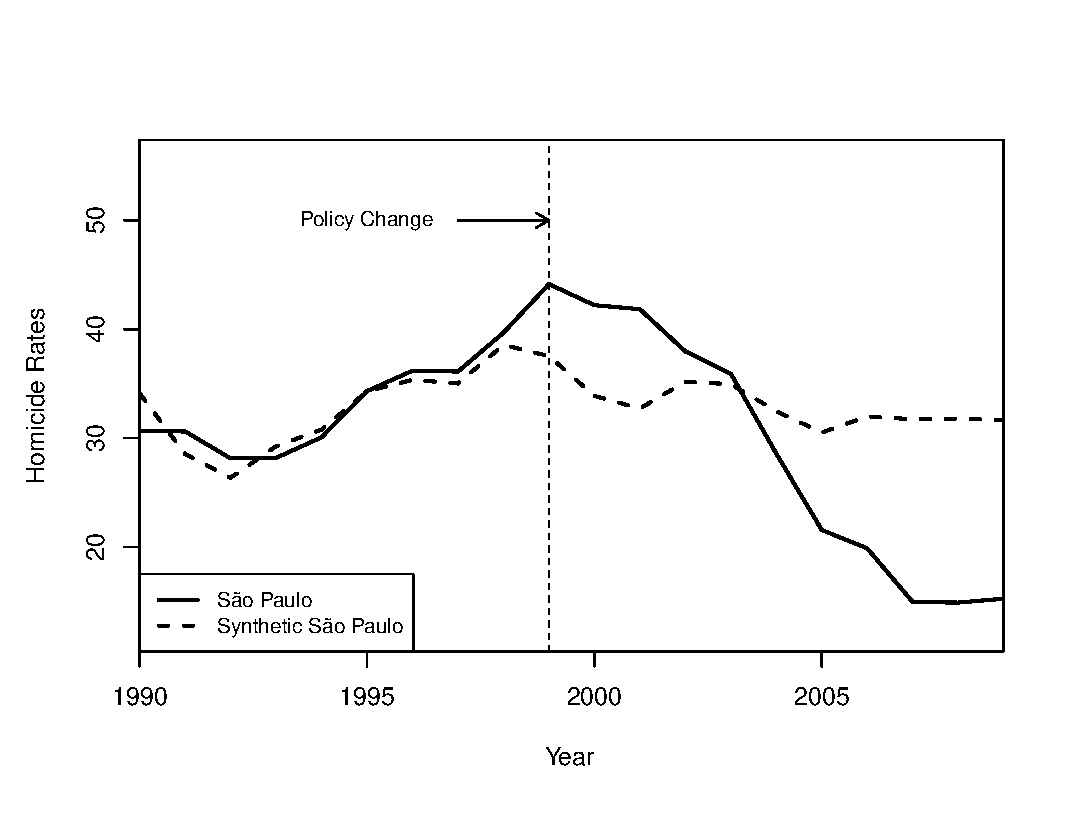
\includegraphics[height=7.5cm]{images/trends.eps}
    \caption{Trends in Homicide Rates: São Paulo versus Synthetic São Paulo}
    \label{fig:figure2}
\end{figure}

Despite the high levels of violence in 1999 -- when the new crime-reducing programme was implemented -- the number of homicides consistently declined until 2009. The trend is indeed monotonic and there is not a single peak in homicide rates after the policies have been put into practice. I interpret that as strong evidence in favour of the public policies. 

\begin{figure}[H]
    \centering
    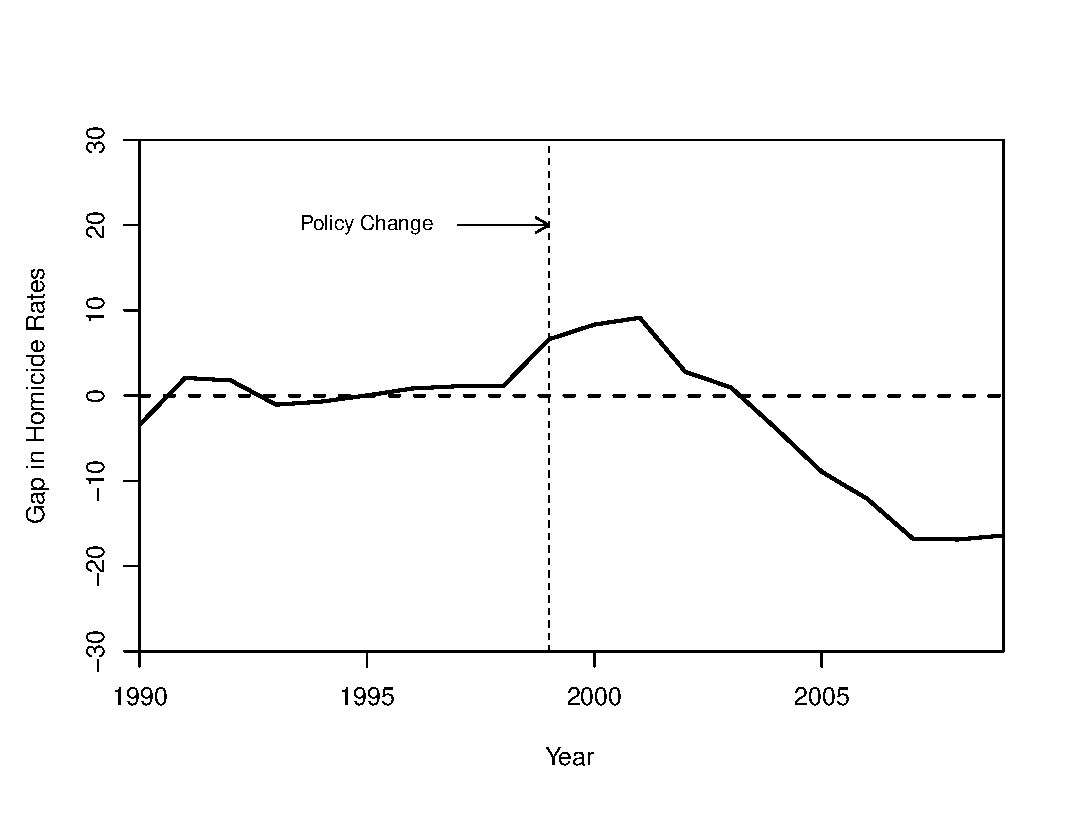
\includegraphics[height=7.5cm]{images/gaps.eps}
    \caption{Homicide Rates Gap between São Paulo and Synthetic São Paulo}
    \label{fig:figure3}
\end{figure}

With respect to the size of the effect, in 1998 the homicide rate in São Paulo was around 40 deaths per 100,000 inhabitants. In 2009 -- the last year for which data are available -- the rate dropped to 15, whereas synthetic São Paulo observed above 30 deaths per 100,000. That means a gap of $-20$ deaths for every 100,000 people in São Paulo in 2009, as can be seen in Figure \ref{fig:figure3}. I estimate that the new policies implemented in São Paulo saved roughly 20,300 lives in the period from 1999 to 2009.\footnote{My estimate of lives saved by the policies implemented in São Paulo is done as follows. I consider the years after policy implementation (1999--2009), then I sum the number of homicides in São Paulo in that period. This gives us 124,077 homicides between 1999 and 2009. I do the same procedure for the synthetic São Paulo; I sum the number of homicides in each state that makes the synthetic control in the period, while adjusting the contribution of each of these states by their respective weights in the synthesis. The number of homicides in synthetic São Paulo between 1999 and 2009 is 144,408. Finally, I subtract the number of homicides in the control by the number of homicides in the treatment. The result is 20,331 lives saved.} It is important to mention that the homicide rate in São Paulo continues to drop by the year, while the same is not happening in the rest of the country. 

\subsection{Robustness Checks}

To further analyse the findings, I run five robustness tests. I first create an `in-time placebo' synthetic control. This test consists of creating a false starting date for the intervention period to check if one could observe false treatment effects in the pre-treatment years \citep{abadie2014}. If that were to be the case, the validity of the main results could be put into question. The result of this placebo test can be seen in Figure \ref{fig:figure4}. When I run the model with 1994 as the year when there was a supposed policy change, the result shows that there is only a minor gap between both lines. In other words, the method does not indicate a definite departure of trends between treatment and control cases. 

\begin{figure}[H]
    \centering
    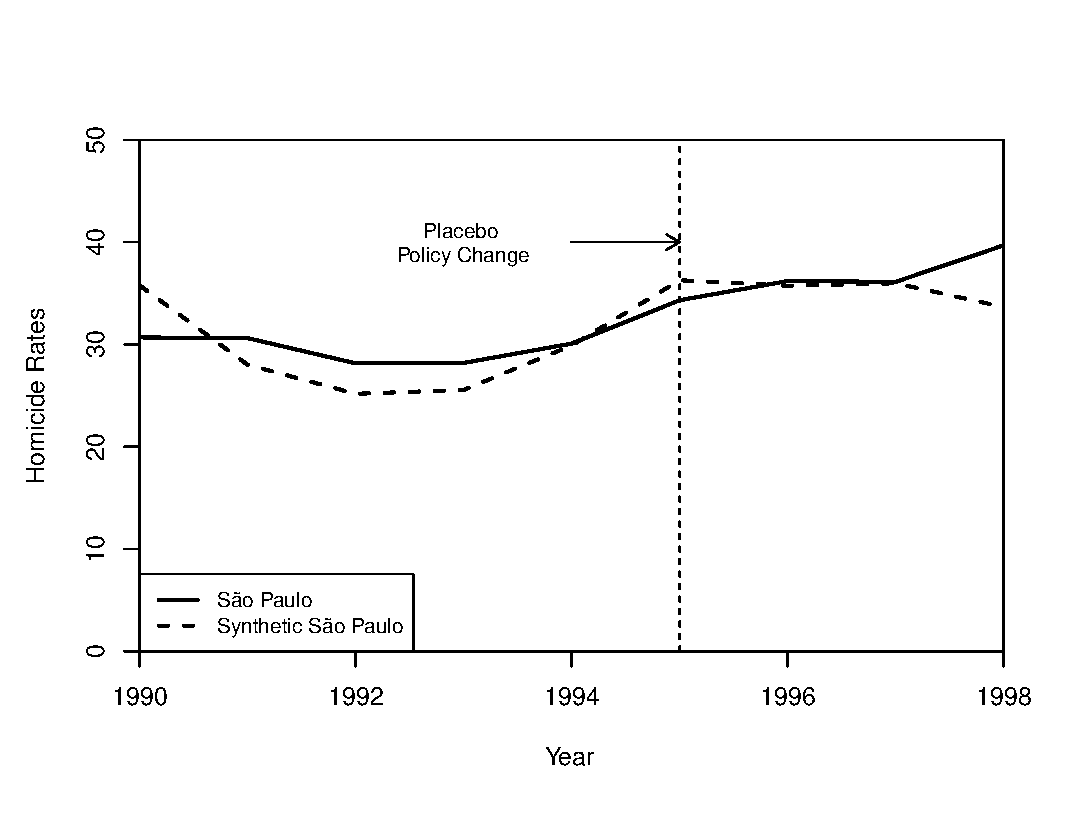
\includegraphics[height=7.5cm]{images/placebo.eps}
    \caption{Placebo Policy Implementation in 1994: São Paulo versus Synthetic São Paulo}
    \label{fig:figure4}
\end{figure}

I also conducted a leave-one-out robustness test. In this test I drop the states composing the synthetic control one at a time. The main goal of this analysis is to evaluate whether a single control state is driving the results. This would suggest that the original synthetic control -- which is composed of five states at a time -- is probably not a reasonable counterfactual. The results of this analysis can be found in Figure \ref{fig:figure5}. We see that the synthetic control (dashed line) is a reasonable amalgam of cases. Also, because the relative positions of treatment and controls are stable across controls, we observe that no control state is biasing the estimates.

\begin{figure}[H]
    \centering
    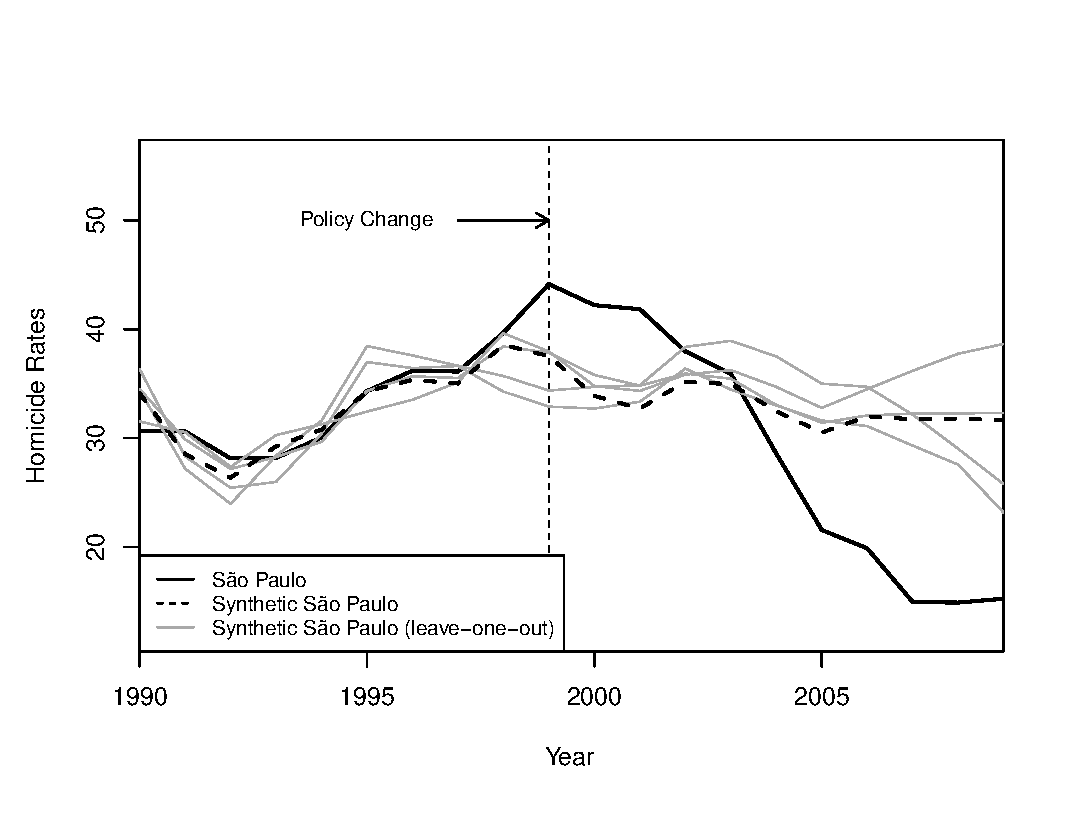
\includegraphics[height=7.5cm]{images/leave-one-out.eps}
    \caption{Leave-One-Out Distribution of the synthetic Control for São Paulo}
    \label{fig:figure5}
\end{figure}

Figure \ref{fig:figure6} shows the difference in homicide rates between the treated units and their synthetic controls. Here I estimate a synthetic control case for São Paulo and for each of the other 26 Brazilian states. This test assesses whether there is any previously unobserved national or regional trend that explains the original results. We observe that in São Paulo the homicide rate gap increases consistently during the treatment period, whereas the lines for the other states are moving randomly. Several lines fail to show any substantial difference between the state line and that of its synthetic counterfactual case. This indicates the results for São Paulo are unlikely to be a result of broader trends.

\begin{figure}[H]
    \centering
    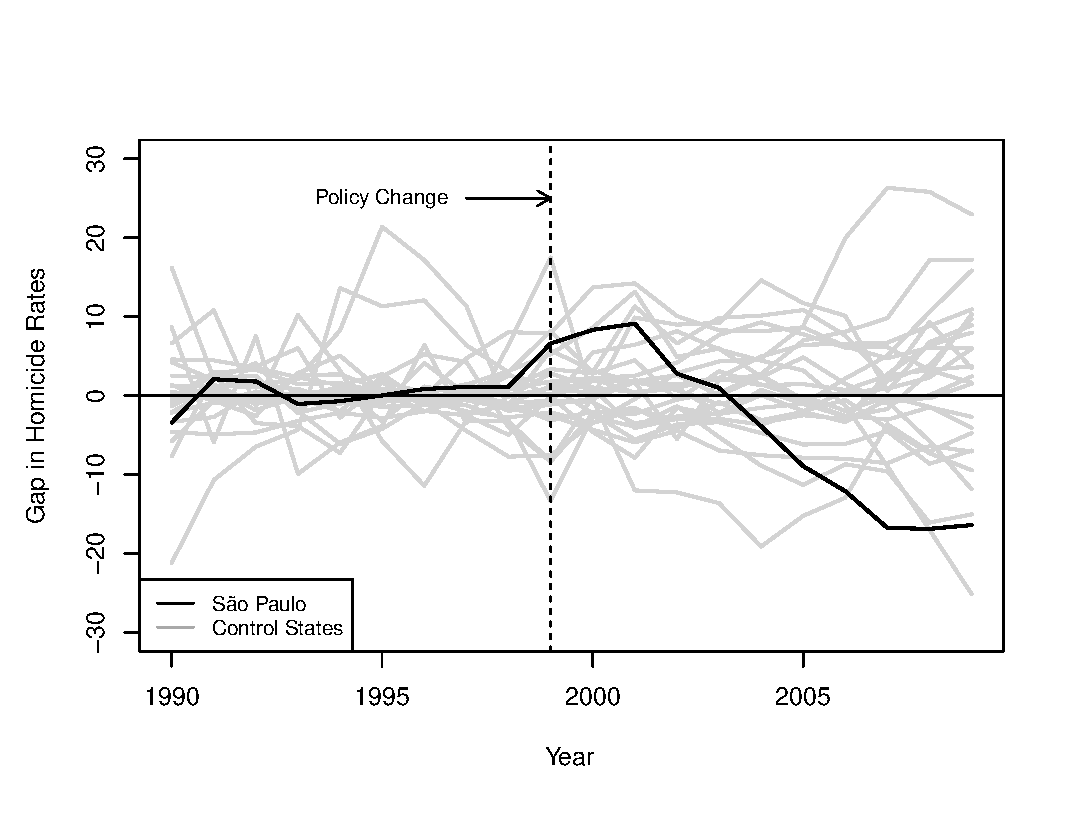
\includegraphics[height=7.5cm]{images/permutation-gaps2.eps}
    \caption{Permutation Test: Homicide Rate Gaps in São Paulo and 26 Control States}
    \label{fig:figure6}
\end{figure}

Figure \ref{fig:figure7} presents the same test displayed in figure \ref{fig:figure6}, but it uses a stricter threshold for the simulated synthetic controls. The graph features cases in which the mean squared prediction error, a measure of goodness-of-fit, is no higher than twice that of São Paulo. That is, only placebos that have good synthetic matches were selected for the analysis \citep[503]{abadie2010}.  In this group, the negative gap for the homicide rate São Paulo is by far the most relevant, providing further evidence for the original findings.

\begin{figure}[H]
    \centering
    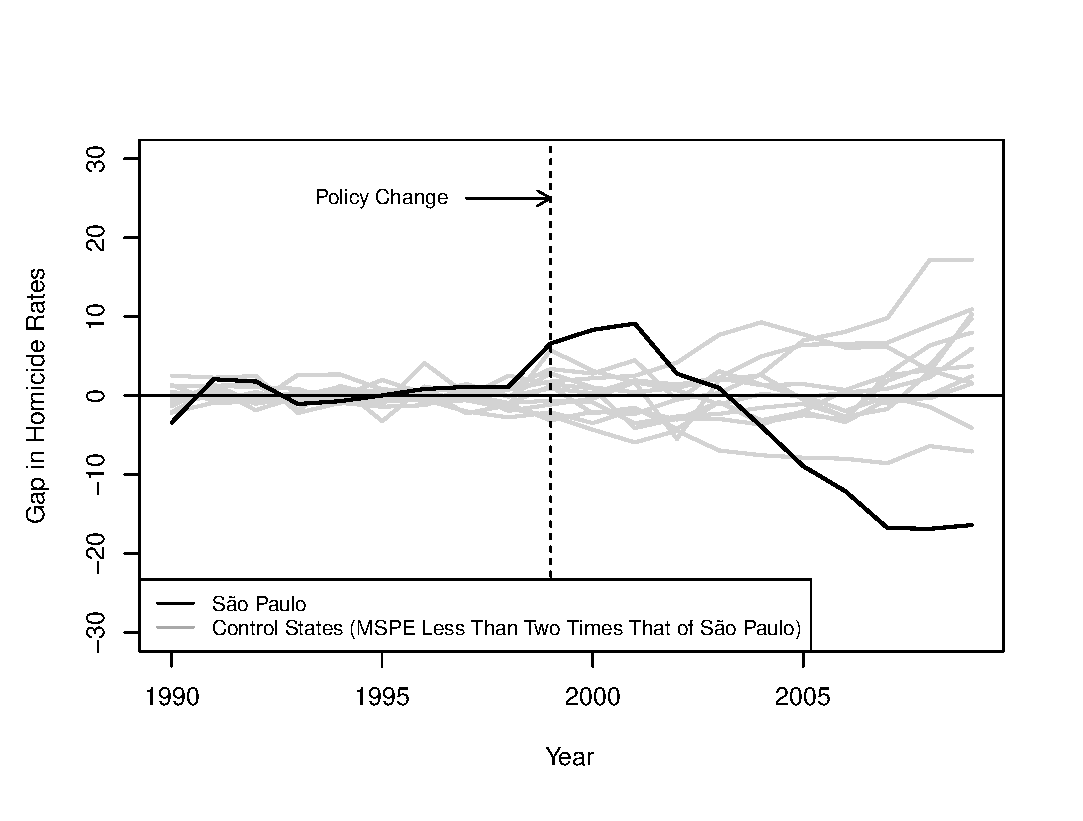
\includegraphics[height=7.5cm]{images/low-mspe.eps}
    \caption{Permutation Test: Homicide Rate Gaps in São Paulo and Selected Control States}
    \label{fig:figure7}
\end{figure}

Lastly, I estimate another synthetic control using a different approach. I employ a Bayesian structural time-series model to verify the stability of the previous results \citep{brodersen2015inferring}. This inference procedure is similar to that described in section \ref{sec:methods} and it also consists of matching pre-treatment values of the unit of interest, São Paulo, to other potential control states. However, in this model only the time trends of the dependent variable are matched. In a sense, this is closer to a traditional differences-in-differences approach, but without the restrictive assumption that the treated and the control cases would follow parallel trends over time \citep[494]{abadie2010}.  

\begin{figure}[H]
    \centering
    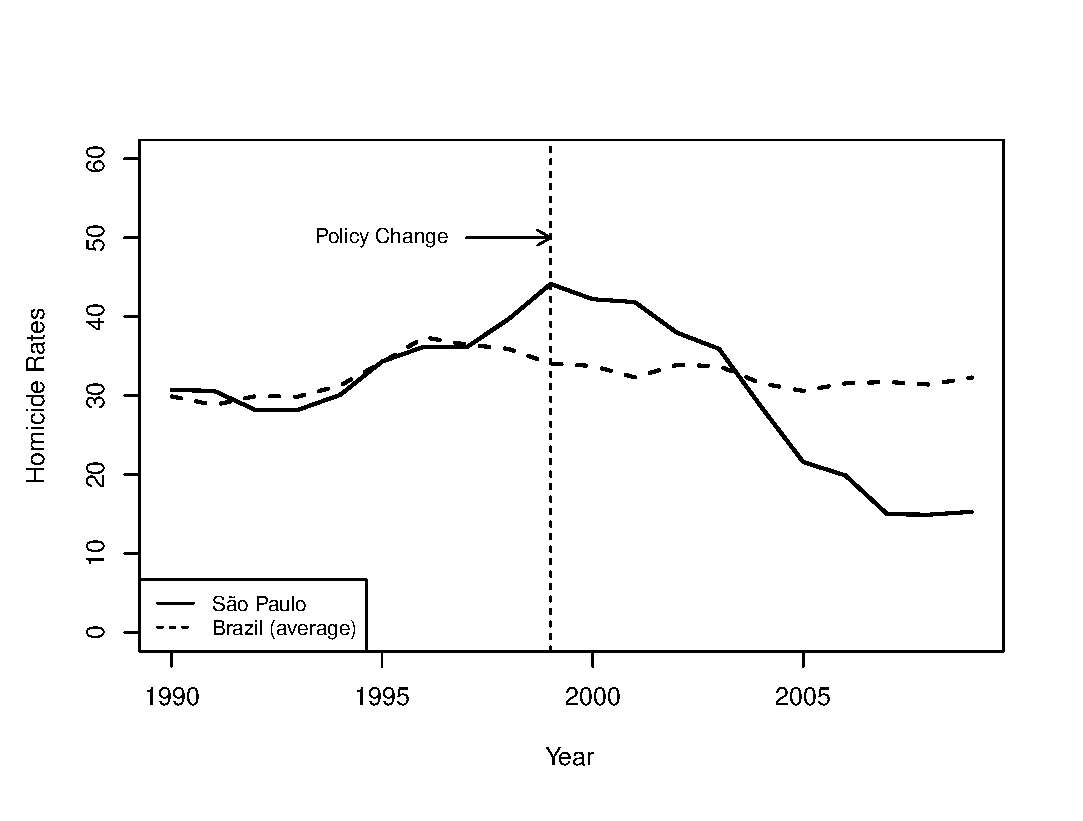
\includegraphics[height=7.5cm]{images/causal-impact.eps}
    \caption{Bayesian Structural Time Series Model: São Paulo and Synthetic São Paulo}
    \label{fig:figure8}
\end{figure}

The model shows that in 2009 we should have expected São Paulo to have a homicide rate equal to 32.3 deaths per 100,000, but we observe only 15.2. Thus, the actual rate in São Paulo corresponds to only 47\% of the expected counterfactual. The method also generates an estimate for the probability of causal effect. The calculations indicate a 96.3\% chance of a causal impact in the period. In this sense, it is unlikely that the results are a statistical fluke.

\section{Conclusion}
\label{sec:conclusion}

As I have hopefully demonstrated, when compared to a synthetic control case, homicide rates were drastically reduced in São Paulo. Although it is not possible to estimate the treatment effect of each specific policy implemented during the 1990s and 2000s, I suggest that their aggregate impact is surely not negligible. If the estimation strategy employed in this paper is correct, the state of São Paulo offers an example that it is feasible to fight crime with targeted policies. This as an encouraging result, as it suggests that governments can make progress in reducing crime with the resources they already have at hand and need not rely exclusively upon structural conditions that are largely beyond their control, such as unemployment, per capita income and inequality. Robustness tests provide further evidence for my findings.

I also argue in favour of the synthetic control method as a tool to evaluate government policies. This approach offers an intuitive way to assess causality claims when there is only a single treated unit and it can be easily applied in a great number of situations. Assuming that there is a reasonable number of potential cases in the `donor pool,' a synthetic control can be meaningfully compared to the actual case. In this way, the technique allows the researcher to use the potential outcomes framework even in unusual conditions.

Future research can extend the present findings in a number of ways. First, it would be interesting to test whether other criminal activities have been affected by the state government policies I mentioned previously. Since property crimes are pervasive in São Paulo, scholars could evaluate the causal link (or lack thereof) between public policies and the incidence of theft or robberies. Unfortunately, several states in Brazil do not publish time-series data for property crime, so I could not use the synthetic control method for that dependent variable. As more data become available, this will create an interesting opportunity for investigation. Secondly, micro-level studies are needed to clarify the mechanisms behind São Paulo's homicide reduction, and isolate direct from indirect effects of each individual policies. Due to the shortage of data on targeted policies, qualitative research may explain what the motivations, successes and shortcomings of São Paulo's recent security measures were. Finally, there are still unresolved questions with regards to the `PCC hypothesis', and this is a promising avenue for future academic work. New research could provide insights into how public policies work and, hopefully, help public authorities to design more effective policies against crime.

\newpage

\section{Appendix} 
\label{sec:synth-appendix}

\subsection{The Synthetic Control Estimator}
\label{sec:synth-estimator}

This appendix presents a formal presentation of the synthetic control estimator. Let $j = 1, \dots, J + 1$ be a series of units in periods $t = 1, \dots, T$. In our case, the units are the 27 Brazilian federal states and the time period spans from 1990 to 2009. Assuming that the first unit, São Paulo, has been exposed to the treatment, we have $J$ control units to be included in the case studies donor pool, \emph{i.e.} the 26 remaining states. We define treatment as the series of post-1999 government anti-crime policies implemented in the São Paulo.

Let $Y_{it}^N$ be the homicide rate that would be observed for unit $i$, São Paulo, at time $t$ with no treatment (1990--1998). Conversely, let $Y_{it}^I$ be the observable outcome for unit $i$ at time $t$ had it been subjected to the treatment in periods $T_{0} + 1$ to $T$ (1999--2009). An important assumption is that the treatment has no effect on unit $i$ before the date of intervention, therefore, the values for São Paulo with and without the policy interventions are the same for the pre-treatment period (1990--1998). In formal terms, $Y_{it}^I = Y_{it}^N$ $\forall t < T_{0}$. The observed outcome is defined by $Y_{it}^I = Y_{it}^N + \alpha_{it}D_{it}$, where $\alpha_{it}$ is the effect of crime-reducing policies on homicide rates, and $D_{it}$ is a binary variable that takes the value of $1$ if we refer to post-intervention period (after 1999) and $0$ otherwise. The goal of this paper is to estimate $\alpha_{it}$, the effect of the treatment (homicide reduction policies), for the state of São Paulo for all $t \geq T_0$, that is, from 1999 to 2009. However, we cannot observe São Paulo \emph{without} those policies, as there is no way for the state to have and not have the intervention at the same time. This is what \citet{holland1986} calls the ``fundamental problem of causal inference'': only one of the outcomes of interest is measurable at any given time.

But although we cannot accurately know how São Paulo would be without the treatment, we can approximate it by using a weighted average of the remaining Brazilian states such that $Y_{it}^N = \delta_{t} + \theta_{t}Z_{i} + \lambda_{t}\mu_{i} + \epsilon_{it}$. In this model, $\delta_{t}$ is an unobserved time-dependent factor common to all cases, $Z_{i}$ is a $(1 \times r)$ vector of observed control variables not affected by the policy, $\theta_{t}$ is a $(r \times 1)$ vector of unknown time-specific parameters, $\lambda_{t}$ is a $(1 \times F)$ vector of unknown common factors to all states, $\mu_{i}$ is a state-specific unobservable variable and $\epsilon_{it}$ represents unobserved transitory shocks with mean $0$ for all units (error term). Basically, what SCM tries to do is to match $Z_{i}$, the control variables, and the pre-treatment $Y_{it}$ of São Paulo (1990--1998) so that $\mu_{i}$ is matched as a result.

Synthetic São Paulo is the weighted average of the other 26 Brazilian states. Thus, it is a $(J \times 1)$ vector of weights $W = (w_2 , \dots, w_{J+1})'$ with $w_j \geq 0$ for $j = 2, \dots, J + 1$ and $w_2 + \dots + w_{J+1} = 1$. Each of the elements included in $W$ represents a specific weighted average of control states, that is, a potential synthetic control for São Paulo. The idea is to select a case that resembles São Paulo as closely as possible. Let $X_{1}$ be a $(k \times 1)$ vector of pre-1999 predictor variables for São Paulo and let $X_{0}$ be a $(k \times J)$ matrix containing the predictor variables for the potential control states. Let $\bar{Y}_{i}^{K_{1}}, \dots, \bar{Y}_{i}^{K_{M}}$ be $M$ linear functions of pre-treatment outcomes $(M \geq F)$. One can choose $w^*$ such that:

$$\sum_{j = 2}^{J + 1} w_{j}^{*} Z_{j} = Z_{1}, \sum_{j = 2}^{J + 1} w_{j}^{*}\bar{Y}_{j}^{K_{1}} = \bar{Y}_{1}^{K_{1}}, \dots, \sum_{j = 2}^{J + 1} w_{j}^{*}\bar{Y}_{j}^{K_{M}} = \bar{Y}_{1}^{K_{M}}$$ 

Consequently, as noted by Abadie and his collaborators (\citeyear{abadie2010}), if $T_{0}$ is sufficiently large when compared to the scale of $\epsilon_{it}$, an approximately unbiased estimator for $\alpha_{1t}$, the effect of public security policies in São Paulo, can be described by:

$$\hat{\alpha}_{1t} = Y_{1t} - \sum_{j = 2}^{J + 1} w_{j}^{*} Y_{jt}$$

for all $t \in \left\{T_{0} + 1, \dots, T \right\}$, that is, after the intervention period (1999--2009). In practice, $W^{*}$ is chosen non-parametrically as to minimise $||X_{1} - X_{0}W||$, subject to the weight constrains. Consider $||X_{1} - X_{0}W||v = \sqrt{(X_{1} - X_{0}W)'V (X_{1} - X_{0}W)}$, where $V$ is a $(k \times k)$ symmetric and semi-definite positive matrix with the relative importance of each assigned homicide rate predictor. From various possible ways of choosing $V$, here I follow the recommendation of \citet{abadie2003} and choose $V^{*}$ as the value of $V$ that minimises the root mean squared prediction error (RMSPE) for homicide rates in the entire pre-treatment period (1990-1998).


\subsection{\texttt{R} Code}
\label{sec:synth-code}

The \texttt{R} code below replicates all statistical analyses and graphs included in this chapter. The original data files as well as the final data set are available at \url{https://github.com/danilofreire/homicides-sp-synth}. 

\singlespacing
\small
\begin{verbatim}
######################
### Data Wrangling ###
######################

# Please set your working directory to the data/ folder

# Clear the workspace
rm(list = ls())

# Load necessary packages
library(reshape2)  # data manipulation

# Dependent variable:
dep <- read.csv("homicide-rates.csv", header = TRUE, skip = 1)

dep.molten <- melt(dep,
                   id.vars = c("Sigla",
                               "Código",
                               "Estado")
                    )

colnames(dep.molten) <- c("abbreviation",
                          "code",
                          "state",
                          "year",
                          "homicide.rates")

dep.molten$year <- as.numeric(substring(dep.molten$year, 2))
\end{verbatim}

\newpage

\begin{verbatim}
# Independent variables
ind1 <- read.csv("state-gdp-capita.csv", header = TRUE, skip = 1)

ind1.molten <- melt(ind1,
                    id.vars = c("Sigla",
                                "Código",
                                "Estado")
                    )

colnames(ind1.molten) <- c("abbreviation",
                           "code",
                           "state",
                           "year",
                           "state.gdp.capita")

ind1.molten$year <- as.numeric(substring(ind1.molten$year, 2))

ind2 <- read.csv("state-gdp-growth-percentage.csv", header = TRUE, skip = 1)

ind2.molten <- melt(ind2,
                    id.vars = c("Sigla",
                                "Código",
                                "Estado")
                    )

colnames(ind2.molten) <- c("abbreviation",
                           "code",
                           "state",
                           "year",
                           "state.gdp.growth.percent")

ind2.molten$year <- as.numeric(substring(ind2.molten$year, 2))

ind3 <- read.csv("gini.csv", header = TRUE, skip = 1)

ind3.molten <- melt(ind3,
                    id.vars = c("Sigla",
                                "Código",
                                "Estado")
                    )

colnames(ind3.molten) <- c("abbreviation",
                           "code",
                           "state",
                           "year",
                           "gini")

ind3.molten$year <- as.numeric(substring(ind3.molten$year, 2))

ind4 <- read.csv("population-projection.csv",
                 header = TRUE,
                 skip   = 1)

ind4.molten <- melt(ind4,
                    id.vars = c("Sigla",
                                "Código",
                                "Estado")
                    )

colnames(ind4.molten) <- c("abbreviation",
                           "code",
                           "state",
                           "year",
                           "population.projection")

ind4.molten$year <- as.numeric(substring(ind4.molten$year, 2))

ind5 <- read.csv("population-extreme-poverty.csv", header = TRUE, skip = 1)

ind5.molten <- melt(ind5,
                    id.vars = c("Sigla",
                                "Código",
                                "Estado")
                    )

colnames(ind5.molten) <- c("abbreviation",
                           "code",
                           "state",
                           "year",
                           "population.extreme.poverty")

ind5.molten$year <- as.numeric(substring(ind5.molten$year, 2))

ind6 <- read.csv("years-schooling.csv", header = TRUE, skip = 1)

ind6.molten <- melt(ind6,
                    id.vars = c("Sigla",
                                "Código",
                                "Estado")
                    )

colnames(ind6.molten) <- c("abbreviation",
                           "code",
                           "state",
                           "year",
                           "years.schooling")

ind6.molten$year <- as.numeric(substring(ind6.molten$year, 2))

# Merges files
data.list <- list(dep.molten,
                  ind1.molten,
                  ind2.molten,
                  ind3.molten,
                  ind4.molten,
                  ind5.molten,
                  ind6.molten)

data1 <- Reduce(function(...) merge(..., all = TRUE), data.list)

# Subset and sort
data2 <- subset(data1, year >= 1990 & year <= 2009)
data2 <- data2[order(data2$state), ]
rownames(data2) <- NULL

# Count missing observations, calculate their percentage
round(sapply(data2, function(x) length(which(is.na(x)))), 2)
round(sapply(data2, function(x) length(which(is.na(x)))/length(x)), 2)

# Linear imputation of missing values.
data2$gini.imp <- approxfun(seq_along(data2$gini), data2$gini)(seq_along(data2$gini))

data2$population.extreme.poverty.imp <- approxfun(seq_along(data2$population.extreme.poverty),
data2$population.extreme.poverty)(seq_along(data2$population.extreme.poverty))

data2$years.schooling.imp <- approxfun(seq_along(data2$years.schooling),
data2$years.schooling)(seq_along(data2$years.schooling))

# Create proportion.extreme.poverty
data2$proportion.extreme.poverty <- data2$population.extreme.poverty.imp / data2$population.projection

# Transform variables to improve interpretation
data2$population.projection.ln <- log(data2$population.projection)

# Save data as df.csv
write.table(data2,
            "df.csv",
            row.names = FALSE,
            col.names = TRUE,
            sep       = ",")
            
#####################
### Data Analysis ###
#####################

# Load necessary packages
library(dplyr) # data manipulation
library(Synth) # models

# Load data
df <- read.csv("df.csv", header = TRUE)

# Prepare data set
df$state <- as.character(df$state) # required by dataprep()

# Plot: Homicide rates for Sao Paulo and Brazil (average)
df1 <- df %>%
        mutate(homicide.sp = ifelse(homicide.rates & state == "São Paulo", homicide.rates, NA)) %>%
        select(year, homicide.sp)

df2 <- df %>%
        mutate(homicide.rates1 = ifelse(homicide.rates & state != "São Paulo", homicide.rates, NA)) %>%
        group_by(year) %>%
        summarise(homicide.br = mean(homicide.rates1, na.rm = TRUE))

setEPS()
postscript(file    = "br.eps",
           horiz   = FALSE,
           onefile = FALSE,
           width   = 7,     # 17.8 cm
           height  = 5.25)  # 13.3 cm

plot(x = df1$year,
     y = df1$homicide.sp,
     type = "l",
     ylim = c(0, 60),
     xlim = c(1990, 2009),
     xlab = "Year",
     ylab = "Homicide Rates",
     cex = 3,
     lwd = 2,
     xaxs = "i",
     yaxs = "i"
)

lines(df2$year,
      df2$homicide.br,
      lty = 2,
      cex = 3,
      lwd = 2)

arrows(1997, 50, 1999, 50,
       col    = "black",
       length = .1)

text(1995, 50,
     "Policy Change",
     cex = .8)

abline(v   = 1999,
       lty = 2)

legend(x = "bottomleft",
       legend = c("São Paulo",
                  "Brazil (average)"),
       lty    = c("solid", "dashed"),
       cex    = .8,
       bg     = "white",
       lwdc(2, 2)
)

invisible(dev.off())

# Prepare data for synth
dataprep.out <-
        dataprep(df,
                 predictors = c("state.gdp.capita",
                                "state.gdp.growth.percent",
                                "population.projection.ln",
                                "years.schooling.imp"
                                ),
                 special.predictors = list(
                         list("homicide.rates", 1990:1998, "mean"),
                         list("proportion.extreme.poverty", 1990:1998, "mean"),
                         list("gini.imp", 1990:1998, "mean")
                         ),
                 predictors.op = "mean",
                 dependent     = "homicide.rates",
                 unit.variable = "code",
                 time.variable = "year",
                 unit.names.variable   = "state",
                 treatment.identifier  = 35,
                 controls.identifier   = c(11:17, 21:27, 31:33, 41:43, 50:53),
                 time.predictors.prior = c(1990:1998),
                 time.optimize.ssr     = c(1990:1998),
                 time.plot             = c(1990:2009)
                 )

# Run synth
synth.out <- synth(dataprep.out)

# Get result tables
print(synth.tables   <- synth.tab(
        dataprep.res = dataprep.out,
        synth.res    = synth.out)
      )

# Plot: Main model
setEPS()
postscript(file    = "trends.eps",
           horiz   = FALSE,
           onefile = FALSE,
           width   = 7,     # 17.8 cm
           height  = 5.25)  # 13.3 cm

path.plot(synth.res    = synth.out,
          dataprep.res = dataprep.out,
          Ylab         = c("Homicide Rates"),
          Xlab         = c("Year"),
          Legend       = c("São Paulo","Synthetic São Paulo"),
          Legend.position = c("bottomleft")
)

abline(v   = 1999,
       lty = 2)

arrows(1997, 50, 1999, 50,
       col    = "black",
       length = .1)

text(1995, 50,
     "Policy Change",
     cex = .8)

invisible(dev.off())

# Main model: gaps plot
setEPS()
postscript(file    = "gaps.eps",
           horiz   = FALSE,
           onefile = FALSE,
           width   = 7,
           height  = 5.25)

gaps.plot(synth.res    = synth.out,
          dataprep.res = dataprep.out,
          Ylab         = c("Gap in Homicide Rates"),
          Xlab         = c("Year"),
          Ylim         = c(-30, 30),
          Main         = ""
)

abline(v   = 1999,
       lty = 2)

arrows(1997, 20, 1999, 20,
       col    = "black",
       length = .1)

text(1995, 20,
     "Policy Change",
     cex = .8)

invisible(dev.off())

## Calculating how many lives were saved during the treatment period

# Weights below retrieved form dataprep.out
# State Code  State Weight  State Name        State Abbreviation
# 42          0.274         Santa Catarina    SC
# 53          0.210         Distrito Federal  DF
# 32          0.209         Espirito Santo    ES
# 33          0.169         Rio de Janeiro    RJ
# 14          0.137         Roraima           RR
# 14          0.001         Pernambuco        PB
# 35          treat         Sao Paulo         SP
\end{verbatim}

\begin{verbatim}
# Get years after policy change
df.2 <- df[which(df$year >= 1999),]

# Calculate total number of deaths in SP
num.deaths.sp <- sum( (df.2$homicide.rates[which(df.2$abbreviation == "SP")])/100000 *
    (df.2$population.projection[which(df.2$abbreviation == "SP")]))

# Calculate estimated number of deaths in Synthetic São Paulo
num.deaths.synthetic.sp <- sum( (0.274 * (df.2$homicide.rates[which(df.2$abbreviation == "SC")])/100000 *
(df.2$population.projection[which(df.2$abbreviation == "SP")]))
                                + (0.210 * (df.2$homicide.rates[which(df.2$abbreviation == "DF")])/100000 *
                                (df.2$population.projection[which(df.2$abbreviation == "SP")]))
                                + (0.209 * (df.2$homicide.rates[which(df.2$abbreviation == "ES")])/100000 *
                                (df.2$population.projection[which(df.2$abbreviation == "SP")]))
                                + (0.169 * (df.2$homicide.rates[which(df.2$abbreviation == "RJ")])/100000 *
                                (df.2$population.projection[which(df.2$abbreviation == "SP")]))
                                + (0.137 * (df.2$homicide.rates[which(df.2$abbreviation == "RR")])/100000 *
                                (df.2$population.projection[which(df.2$abbreviation == "SP")]))
                                + (0.001 * (df.2$homicide.rates[which(df.2$abbreviation == "PB")])/100000 *
                                (df.2$population.projection[which(df.2$abbreviation == "SP")]))
                                )

lives.saved <- num.deaths.synthetic.sp - num.deaths.sp
lives.saved # Between 1999 and 2009

########################
### Robustness Tests ###
########################

# Prepare data set
df$state <- as.character(df$state) # required by dataprep()

## Placebo Test -- Control ends in 1994
dataprep.out1 <-
        dataprep(df,
                 predictors = c("state.gdp.capita",
                                "state.gdp.growth.percent",
                                "population.projection.ln",
                                "years.schooling.imp"
                 ),
                 special.predictors = list(
                         list("homicide.rates", 1990:1994, "mean"),
                         list("proportion.extreme.poverty", 1990:1994, "mean"),
                         list("gini.imp", 1990:1994, "mean")
                 ),
                 predictors.op = "mean",
                 dependent     = "homicide.rates",
                 unit.variable = "code",
                 time.variable = "year",
                 unit.names.variable   = "state",
                 treatment.identifier  = 35,
                 controls.identifier   = c(11:17, 21:27, 31:33, 41:43, 50:53),
                 time.predictors.prior = c(1990:1994),
                 time.optimize.ssr     = c(1990:1994),
                 time.plot             = c(1990:1998))

# Run synth
synth.out1 <- synth(dataprep.out1)

# Get result tables
print(synth.tables   <- synth.tab(
        dataprep.res = dataprep.out1,
        synth.res    = synth.out1)
      )

# Placebo test: graph
setEPS()
postscript(file    = "placebo.eps",
           horiz   = FALSE,
           onefile = FALSE,
           width   = 7,
           height  = 5.25)

path.plot(synth.res       = synth.out1,
          dataprep.res    = dataprep.out1,
          Ylab            = c("Homicide Rates"),
          Xlab            = c("Year"),
          Legend          = c("São Paulo","Synthetic São Paulo"),
          Legend.position = c("bottomleft"),
          Ylim            = c(0, 50)
)

abline(v   = 1995,
       lty = 2)

arrows(1994, 40, 1995, 40,
       col    = "black",
       length = .1)

text(1993, 40,
     "Placebo \nPolicy Change",
     cex = .8)

invisible(dev.off())

## Leave-one-out

# Loop over leave one outs
storegaps <- matrix(NA, length(1990:2009), 4)

colnames(storegaps) <- c(14, 33, 42, 53) # RR, RJ, SC, DF
co <- unique(df$code)
co <- co[-25]

for(k in 1:4){

        # Data prep for training model
        omit <- c(14, 33, 42, 53)[k]

        # Prepare data for synth
        dataprep.out2 <-
                dataprep(df,
                         predictors = c("state.gdp.capita",
                                        "state.gdp.growth.percent",
                                        "population.projection.ln",
                                        "years.schooling.imp"
                         ),
                         special.predictors = list(
                                 list("homicide.rates", 1990:1998, "mean"),
                                 list("proportion.extreme.poverty", 1990:1998, "mean"),
                                 list("gini.imp", 1990:1998, "mean")
                         ),
                         predictors.op = "mean",
                         dependent     = "homicide.rates",
                         unit.variable = "code",
                         time.variable = "year",
                         unit.names.variable   = "state",
                         treatment.identifier  = 35,
                         controls.identifier   = co[-which(co==omit)],
                         time.predictors.prior = c(1990:1998),
                         time.optimize.ssr     = c(1990:1998),
                         time.plot             = c(1990:2009)
                )

        # Run synth
        synth.out2 <- synth(dataprep.out2)

        storegaps[,k] <- (dataprep.out2$Y0%*%synth.out2$solution.w)
} # Close loop over leave one outs

# Leave-one-out: graph
setEPS()
postscript(file    = "leave-one-out.eps",
           horiz   = FALSE,
           onefile = FALSE,
           width   = 7,
           height  = 5.25)

path.plot(synth.res    = synth.out,
          dataprep.res = dataprep.out,
          Ylab         = c("Homicide Rates"),
          Xlab         = c("Year"),
          Legend       = c("São Paulo","Synthetic São Paulo"),
          Legend.position = c("bottomleft"))

abline(v   = 1999,
       lty = 2)

arrows(1997, 50, 1999, 50,
       col    = "black",
       length = .1)

text(1995, 50,
     "Policy Change",
     cex = .8)

for(i in 1:4){
        lines(1990:2009,
              storegaps[,i],
              col = "darkgrey",
              lty = "solid")
}

lines(1990:2009,
      dataprep.out$Y0plot %*% synth.out$solution.w,
      col = "black",
      lty = "dashed",
      lwd = 2)

legend(x = "bottomleft",
       legend = c("São Paulo",
                  "Synthetic São Paulo",
                  "Synthetic São Paulo (leave-one-out)"
       ),
       lty    = c("solid", "dashed", "solid"),
       col    = c("black", "black", "darkgrey"),
       cex    = .8,
       bg     = "white",
       lwdc(2, 2, 1)
)

invisible(dev.off())

## Permutation test
states <- c(11:17, 21:27, 31:33, 35, 41:43, 50:53)

# Prepare data for synth
results <- list()
results_synth <- list()
gaps <- list()

for (i in states) {
    dataprep.out <-
            dataprep(df,
                     predictors = c("state.gdp.capita",
                                    "state.gdp.growth.percent",
                                    "population.projection.ln",
                                    "years.schooling.imp"
                                    ),
                     special.predictors = list(
                             list("homicide.rates", 1990:1998, "mean"),
                             list("proportion.extreme.poverty", 1990:1998, "mean"),
                             list("gini.imp", 1990:1998, "mean")
                             ),
                     predictors.op = "mean",
                     dependent     = "homicide.rates",
                     unit.variable = "code",
                     time.variable = "year",
                     unit.names.variable   = "state",
                     treatment.identifier  = i,
                     controls.identifier   = states[which(states!=i)],
                     time.predictors.prior = c(1990:1998),
                     time.optimize.ssr     = c(1990:1998),
                     time.plot             = c(1990:2009)
                     )
    results[[as.character(i)]] <- dataprep.out
    results_synth[[as.character(i)]] <- synth(results[[as.character(i)]])
    gaps[[as.character(i)]] <- results[[as.character(i)]]$Y1plot - (results[[as.character(i)]]$Y0plot %*%
    results_synth[[as.character(i)]]$solution.w)

}

## Permutation test
setEPS()
postscript(file    = "permutation-gaps2.eps",
           horiz   = FALSE,
           onefile = FALSE,
           width   = 7,
           height  = 5.25)

plot(1990:2009,
     ylim = c(-30, 30),
     xlim = c(1990,2009),
     ylab = "Gap in Homicide Rates",
     xlab = "Year"
)

for (i in states) {
        lines(1990:2009,
              gaps[[as.character(i)]],
              col = "lightgrey",
              lty = "solid",
              lwd = 2
        )
}

lines(1990:2009,
      gaps[["35"]], # São Paulo
      col = "black",
      lty = "solid",
      lwd = 2
)

abline(v   = 1999,
       lty = 2)
\end{verbatim}

\newpage 

\begin{verbatim}
abline(h   = 0,
       lty = 1,
       lwd = 1)

arrows(1997, 25, 1999, 25,
       col    = "black",
       length = .1)

text(1995, 25,
     "Policy Change",
     cex = .8)

legend(x = "bottomleft",
       legend = c("São Paulo",
                  "Control States"),
       lty  = c("solid", "solid"),
       col  = c("black", "darkgrey"),
       cex  = .8,
       bg  = "white",
       lwdc(2, 2, 1)
)

invisible(dev.off())

# Permutation graph: states with MSPE no higher than 2x São Paulo's
low.mspe <- c(13, 15, 17, 21, 23, 24, 25, 31, 41:43, 53)

setEPS()
postscript(file    = "low-mspe.eps",
           horiz   = FALSE,
           onefile = FALSE,
           width   = 7,
           height  = 5.25)

plot(1990:2009,
     ylim = c(-30, 30),
     xlim = c(1990,2009),
     ylab = "Gap in Homicide Rates",
     xlab = "Year"
)

for (i in low.mspe) {
lines(1990:2009,
      gaps[[as.character(i)]],
      col = "lightgrey",
      lty = "solid",
      lwd = 2
      )
}

lines(1990:2009,
      gaps[["35"]], # São Paulo
      col = "black",
      lty = "solid",
      lwd = 2
      )

abline(v   = 1999,
       lty = 2)

abline(h   = 0,
       lty = 1,
       lwd = 1)

arrows(1997, 25, 1999, 25,
       col    = "black",
       length = .1)

text(1995, 25,
     "Policy Change",
     cex = .8)

legend(x = "bottomleft",
       legend = c("São Paulo",
                  "Control States (MSPE Less Than Two Times That of São Paulo)"),
       lty    = c("solid", "solid"),
       col    = c("black", "darkgrey"),
       cex    = .8,
       bg     = "white",
       lwdc(2, 2, 1)
)

invisible(dev.off())

## CausalImpact
# Uncomment the lines below to install necessary packages
# install.packages(c("devtools", "dtw"))
# library(devtools)
# install_github("google/CausalImpact")
# install_github("klarsen1/MarketMatching", build_vignettes=TRUE)

# Load packages
library(CausalImpact)
library(MarketMatching)

# Prepare data
df$year2 <- as.Date(paste(df$year, sep = "", "-01-01"))

# Estimate model
mm <- best_matches(data=df,
                   id_variable="code",
                   date_variable="year2",
                   matching_variable="homicide.rates",
                   parallel=TRUE,
                   warping_limit=1, # warping limit=1
                   dtw_emphasis=1, # rely only on dtw for pre-screening
                   matches=5, # request 5 matches
                   start_match_period="1990-01-01",
                   end_match_period="1998-01-01")

# View best matches
subset(mm$BestMatches, code == 35) # SP

# Results
results <- MarketMatching::inference(matched_markets = mm,
                                     test_market = "35",
                                     end_post_period = "2009-01-01")

# Predictions
results$Predictions

# Plot results
results$PlotActualVersusExpected +
        ggtitle("São Paulo versus Synthetic São Paulo") + theme_bw() +
        geom_line(aes(results$PlotActualVersusExpected$data$test_market),colour="#000099")
results$PlotCumulativeEffect

# Graph
setEPS()
postscript(file    = "causal-impact.eps",
           horiz   = FALSE,
           onefile = FALSE,
           width   = 7,     # 17.8 cm
           height  = 5.25)  # 13.3 cm

plot(x = (1990:2009),
     y = as.numeric(results$Predictions$Response),
     type = "l",
     ylim = c(0, 60),
     xlim = c(1990, 2009),
     xlab = "Year",
     ylab = "Homicide Rates",
     cex = 3,
     lwd = 2)

lines(x = (1990:2009),
      y = as.numeric(results$Predictions$Predicted),
      type = "l",
      lty = 2,
      cex = 3,
      lwd = 2)

arrows(1997, 50, 1999, 50,
       col    = "black",
       length = .1)

text(1995, 50,
     "Policy Change",
     cex = .8)

abline(v   = 1999,
       lty = 2)

legend(x = "bottomleft",
       legend = c("São Paulo",
                  "Brazil (average)"),
       lty    = c("solid", "dashed"),
       cex    = .8,
       bg     = "white",
       lwdc(2, 2)
)

invisible(dev.off())
\end{verbatim}

\doublespacing
\normalsize